\subsection{Environment Capture}
In order to capture the environment, we rely on the KinectFusion\cite{newcombe2011kinectfusion}  algorithm as our environment is static and we require the algorithm to be realtime. There are two main implementations of KinectFusion available. The Kinect Development Toolkit for Windows comes with an API to access KinectFusion. They do not provide source code but let the developer access KinectFusion in a limited matter. Also this version has only been demonstrated on small volumes and the tracking is not very stable when using large volumes with small voxel denisty. Given a camera pose and a camera matrix, the API allows the user to render the scene from that camera.\\
\begin{figure}[ht]
	\centering
	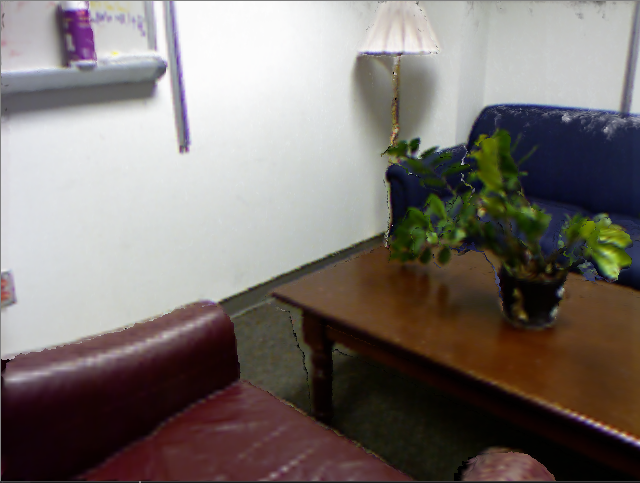
\includegraphics[width=3.0in]{images/scene2.png}
	\caption{A scene capture from Kinect}
	\label{fig:kinectFusionOut}
\end{figure}
The other popular implementation is KinFu that comes with PCL. This contains extensions on KinectFusion that enable it to work in large areas. It does so by decomposing the environment into chunks that can be uploaded to the GPU. This allows it to reconstruct a large volume while maintaining a high voxel density.This results in more robust tracking.  